\begin{minipage}[bt]{0.5\linewidth}
%==============================================================
\item Seja $A = \{a, b, c, d, e, f\}$ o conjunto das retas da figura ao lado :
Para a relação 
\[
xRy\ \Leftrightarrow\ x\  \mbox{é paralela a}\ y
\]
Mostre que $R$ é uma relação de equivalência.
%==============================================================
\end{minipage}
%==============================================================
\hspace{0.04\textwidth}
%==============================================================
\begin{minipage}[h]{0.4\linewidth}
\centering
%==============================================================
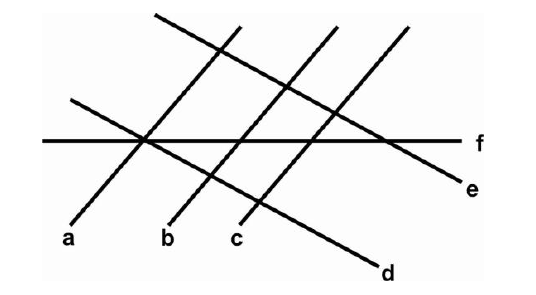
\includegraphics[scale=.5]{fig1-q49.png}
%==============================================================
%\caption{Histograma Exemplo~\ref{exe1-moda}} %
\end{minipage}
%\end{figure}
